My educational journey, influenced by remarkable and dedicated mentors, has led me to value the transformative power of effective teaching. I strive for a pedagogy that balances engagement, conveyance, and inspiration, guided by five introspective questions when creating course materials:
\begin{enumerate*}[label=\arabic*)]
    \item What insights will students gain from the synchronization of spoken words and slides?
    \item What about when they independently examine the slide content at lecture pace?
    \item What are their takeaways when revisiting the slides after class?
    \item How can I ensure consistency in key takeaways across various learning contexts?
    \item How can I structure slides to effectively convey key messages without direct reading?
\end{enumerate*}
These practices have shaped my teaching philosophy, which emphasizes the effective use of visualization.

\begin{wrapfigure}{r}{0.29\textwidth}%
    \centering
    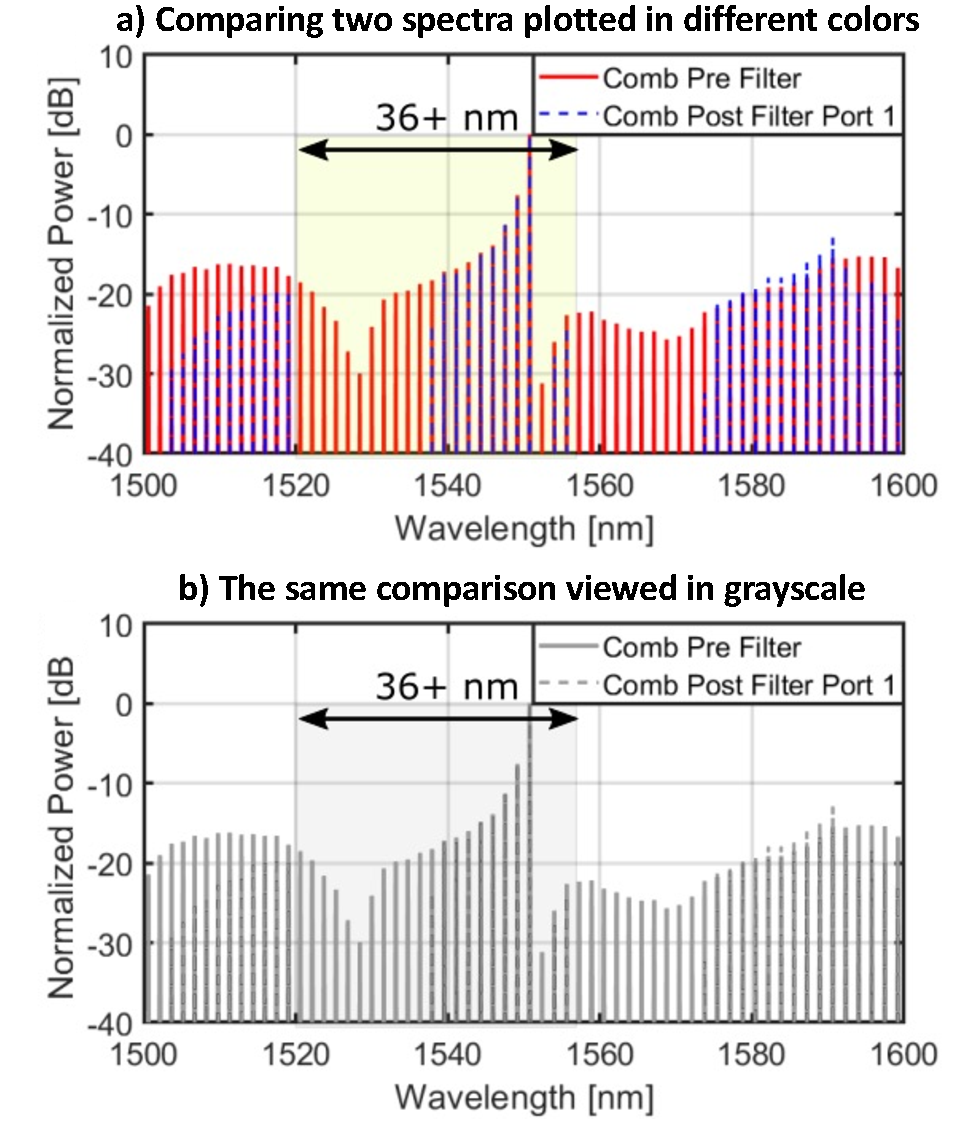
\includegraphics[width=\linewidth]{../../fig/color_vertical.pdf}
    \caption{Example of non-inclusive color use: \textbf{a)}~two spectra distinguishable with normal color vision; \textbf{b)}~indistinguishable as possibly rendered by impaired color vision.}
    \label{fig:color}
\end{wrapfigure}

\paragraph{Teaching Philosophy}
Visualization is central to my instructional approach, leveraging the human brain's rapid image processing ability, reportedly surpassing text interpretation by 6x\textendash 600x\footnote{
    Despite the discrepancy with the unfounded meme claiming 60,000x, as called out in \emph{Research: Is a Picture Worth 1,000 Words Or 60,000 Words in Marketing?} (\url{https://www.emailaudience.com/research-picture-worth-1000-words-marketing/}), this is still substantial enough to warrant extra attention to the use of visualization in teaching.
}.
This enables more efficient extraction of information from slide content, allowing for profound engagement. In STEM education, where theories and equations can become overwhelming, visualization serves to translate intricate ideas into comprehensible and memorable images. It also addresses the challenge of conveying essential concepts without merely reading from slides\textemdash a practice that hinders critical thinking. Beyond classroom benefits, effectively visualizing data and concepts is an indispensable skill for students' academic pursuits and research careers. Building on this, I address the challenge of ensuring consistent takeaways in different learning contexts by integrating concise bullet points alongside visuals.

\paragraph{Inclusive Teaching}
Informed by my personal experience with minor color vision deficiency, I design visual materials with inclusivity in mind. For example, as shown in Fig.~\ref{fig:color}, using color as the sole differentiator between two spectra being compared can be challenging for those with color vision impairments. The seemingly surprising prevalence of color blindness, affecting approximately 8\% of males and 0.5\% of females\footnote{
    \emph{Types of Colour Blindness} (\url{https://www.colourblindawareness.org/colour-blindness/types-of-colour-blindness/})
}, virtually guarantees that any moderately sized classroom will have students with a form of color vision deficiency. To ensure accessibility for all, I always use multiple modes of differentiation, such as patterns, textures, and annotations. My commitment to inclusivity further extends to all diversity and accessibility aspects in education. Understanding the varied cultural, personal, and educational backgrounds of students, I aim to create a classroom environment that is physically, cognitively, and culturally welcoming, employing inclusive language and diverse examples in my teaching materials, practices that will be regularly reviewed for adherence.


\paragraph{Teaching Interest}
Aligned with the esteemed curriculum of \appSchool{}'s \appDept{}, I am eager to contribute by teaching a range of courses that intersect with my expertise,
\rsCustom{}

\paragraph{Mentoring}
My mentoring philosophy extends beyond knowledge sharing and intellectual guidance. I aim to provide holistic support for students in both academic and professional growth, through creating a collaborative research environment that encourages them to excel academically, uphold professionalism, and pursue their research interests towards becoming independent researchers. My postdoctoral experience at the Columbia University involved guiding several Ph.D. students to key achievements, such as publishing papers as lead authors at premier conferences and obtaining their initial industry positions. I look forward to further developing and applying these mentorship practices at the \appSchool{}.

\paragraph{Post\textendash COVID-19 Considerations}

In response to the post\textendash COVID-19 new norm of hybrid teaching and research, I have adapted and am ready to further refine my approaches to meet the evolving challenges. Plans include enhancing slides with necessary annotations and animations to compensate for the reduced interaction of physical whiteboard sessions. Furthermore, I intend to organize regular coffee hours or lunch meetings to facilitate in-person discussions when possible, following university guidelines. This adaptability is essential in the changing educational landscape, and I am committed to continually innovating my teaching and mentoring methods to ensure accessible and effective education for all students.